
\section{Machine Learning}

Machine learning (ML) is the field of study of mathematical models that can automatically learn patterns from sample data, known as \textit{training} data, in order to make predictions for unseen data.
Regression and classification are two common types of machine learning application~\cite{goodfellow16}.

Regression concerns the prediction of a numerical value given some inputs, where an ML model learns the relationship between the outcome variable and one or more input features.
Figure~\ref{fig:ml-regression} illustrates an example of a regression model.
Based on the sample data, a curve is fitted, minimising the overall error between the sample data and the curve.
This curve represents the model that can be used to estimate the outcome variable for an unseen feature data.

\begin{figure}[h]
  \centering
  \begin{subfigure}{.32\textwidth}
    \center
    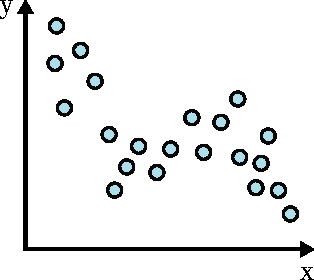
\includegraphics[scale=0.8]{src/background/figs/ml-regression-sample}
    \caption{Sample data.}
    \label{fig:ml-regression-sample}
  \end{subfigure}
  \begin{subfigure}{.32\textwidth}
    \center
    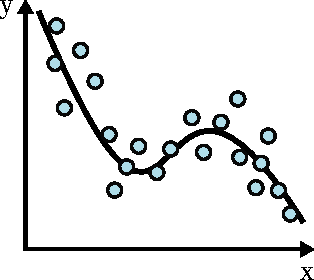
\includegraphics[scale=0.8]{src/background/figs/ml-regression-fitted}
    \caption{Fitted curve.}
    \label{fig:ml-regression-fitted}
  \end{subfigure}
  \begin{subfigure}{.32\textwidth}
    \center
    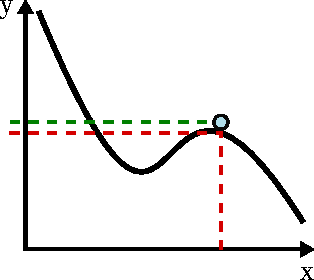
\includegraphics[scale=0.8]{src/background/figs/ml-regression-model}
    \caption{Model.}
    \label{fig:ml-regression-model}
  \end{subfigure}
  \caption{
    An illustration of a regression model using machine learning.
    A regression model use the sample data to learn a function that maps the input features to an outcome numerical variable.
  }
  \label{fig:ml-regression}
\end{figure}

Classification concerns the prediction of a categorical label given some inputs, where an ML model learns the relationship between a finite set of labels and one or more input features.
The training of a classifier requires inputs for which the category is known, called labelled training data.
Figure~\ref{fig:ml-classifier} illustrates an example of a binary classification model.
Based on the sample data, a curve is fitted, minimising the number of misclassification.
This curve represents the model that can be used to predict the category of unseen feature data.

% In this type of task, the computer program is asked to specify which of k categories some input belongs to. To solve this task, the learning algorithm is usually asked to produce a function f:Rn→ {1, . . . , k}. When y=f(x), the model assigns an input described by vector x to a category identified by numeric code y. There are other variants of the classification task, for example, where f outputs a probability distribution over classes. An example of a classification task is object recognition, where the input is an image (usually described as a set of pixel brightness values), and the output is a numeric code identifying the object in the image.

\begin{figure}[h]
  \centering
  \begin{subfigure}{.32\textwidth}
    \center
    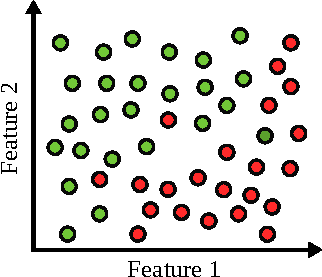
\includegraphics[scale=0.8]{src/background/figs/ml-classifier-sample}
    \caption{Sample data.}
    \label{fig:ml-classifier-sample}
  \end{subfigure}
  \begin{subfigure}{.32\textwidth}
    \center
    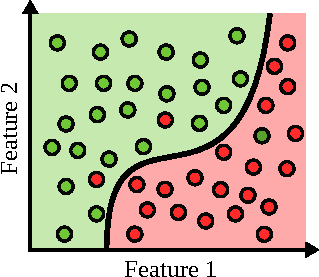
\includegraphics[scale=0.8]{src/background/figs/ml-classifier-fitted}
    \caption{Fitted curve.}
    \label{fig:ml-classifier-fitted}
  \end{subfigure}
  \begin{subfigure}{.32\textwidth}
    \center
    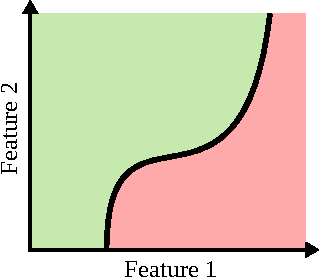
\includegraphics[scale=0.8]{src/background/figs/ml-classifier-model}
    \caption{Model.}
    \label{fig:ml-classifier-model}
  \end{subfigure}
  \caption{
    An illustration of a classification model using machine learning.
    A regression model use the sample data to learn a function that maps the input features to an outcome numerical variable.
  }
  \label{fig:ml-classifier}
\end{figure}

\subsection{Neural Networks}

Machine is commonly seen as a subset of artificial intelligence and a superset of deep-learning (DL), which is a family of machine learning methods based on artificial neural networks.
Artificial neural networks (ANNs) are machine learning models that were vaguely inspired by the biological neural networks.
These models are composed of artificial neurons, which are essentially mathematical functions known as \textit{activation functions}, mapping inputs to a single output that can be fed to multiple other neurons.
These neurons are connected by weighted edges, forming a graph, i.e., the artificial neural network.

\subsubsection{Feed-Forward Neural Networks}

A feed-forward neural networks is a simple but powerful neural network architecture where information flows through the layers in only one direction, namely, forward, as illustrated in Figure~\ref{fig:ML-feed-forward-network}.
Feed-forward neural networks with multiple layers work as universal function approximators of any bounded continuous function to arbitrary precision~\cite{hornik91,lu17}.
Essentially, this model defines a mapping $\mathbf{y} = f(\mathbf{x};\mathbf{\theta})$, were $\mathbf{\theta}$ represents the parameters that are learnt, optimising the function approximation.

The architecture of the feed-forward network is a direct acyclic graph, where the neurons are grouped in layers, forming what is also known as a multi-layer perceptrons.
The neurons are connected only across layers, i.e., the neurons in one layer are connect to the neurons following layer.
The first layer is the input layer, with $x_i$ being the input variables, and the last layer is the output layer, with $y_i$ being the output variables.
All other layers in between are the hidden layers, for which there are no known ground truth values.
The value for these hidden layers are computed using a specific activation function that is chosen per layer.
The number of layers of the architecture is known as the depth of the model, with the final layer being the output layer.
When designing the architecture of a feed-forward neural network, in addition to the activation functions in each layer, we must also decide on how many layers the network should contain, how these layers should be connected to each other, and how many units should be in each layer~\cite{goodfellow16}.

\begin{figure}[h]
  \centering
  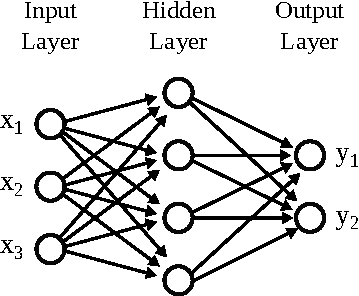
\includegraphics[scale=0.85]{src/background/figs/ML-feed-forward-network.pdf}
  \caption{Example of an artificial neural network with multiple layers of neurons. Each circle represents an artificial neuron. Adjacent layers of neurons are fully connected.}
  \label{fig:ML-feed-forward-network}
\end{figure}

%\paragraph{Activation Function}

%A common activation function in feed forward networks are sigmoids.
%Two of the sigmoid functions commonly used are the logistic and the hyperbolic tangent function.
%The logistic function is defined as $\phi(x) = \frac{1}{1+e^{-x}}$ and the hyperbolic tangent function is defined as 

\paragraph{Back-propagation}

Neural networks can use a large variety of learning algorithms.
Learning consists of finding weights for the parameters in order to minimise the prediction error.
The most widely used learning technique is known as back-propagation~\cite{rumelhart88,goodfellow16}.

Learning in deep neural networks requires computing the gradients of complicated functions.
We present the back-propagation algorithm and its modern generalizations, which can be used to efficiently compute these gradients.

Typically, this algorithm initialises the weights with random values.
During the training process, a batch of samples is propagated through the network in a feed-forward way.
The outputs of the network is then compared against the true values, computing a prediction error.
The error function is chosen as part of the design of the network, as the appropriate function depends on the task.
This prediction error is propagated back to each individual neuron. %, using the learning rule below:

For each neuron, it computes what the output should have been and updates the weights of the neuron accordingly.
Finally, this process is repeated for different batches until it converges, producing a prediction error below a certain threshold.

\subsubsection{Recurrent Neural Networks}

Recurrent neural networks (RNNs) are a family of neural networks for processing sequential.
Most recurrent networks can process sequences of variable length, which is impractical for networks without sequence-based specialisation.
In order to process input sequences of variable length, RNNs have feed-back connections in which outputs of the model are fed back into itself, forming a cycle (or recursion) in the network~\cite{goodfellow16}.

Two important RNNs are long short-term memory and networks based on the gated recurrent unit.

\paragraph{Long Short-Term Memory}

Long short-term memory~\cite{Graves12} (LSTM) is an RNN architecture designed to overcome the vanishing gradients problem.
The LSTM augments RNN design with the addition of a cell for storing information, and three gates which control the flow of information into and out of the cell.

Long short-term memory (LSTM) is an RNN architecture designed to overcome the vanishing gradients problem.
The LSTM augments RNN design with the addition of a cell for storing information, and three gates which control the flow of information into and out of the cell.

\paragraph{Gated Recurrent Units}

Gated recurrent units (GRUs) are a gating mechanism in recurrent neural networks, introduced in 2014 by Kyunghyun Cho et al. The GRU is like a long short-term memory (LSTM) with a forget gate but has fewer parameters than LSTM, as it lacks an output gate. GRU's performance on certain tasks of polyphonic music modelling, speech signal modelling and natural language processing was found to be similar to that of LSTM. GRUs have been shown to exhibit even better performance on certain smaller and less frequent datasets.

\subsection{Evaluation}

\subsubsection{Evaluating Binary Classifiers}

The goal of a binary classifier is to correctly assign one out of two labels for a given input.
Without loss of generality, we can assume the two labels are ``positive'' and ``negative''.
Figure~\ref{fig:evaluation-classification} represents all four possibilities for the labelling produced by a binary classification.
True positives refer to correct classification of positive labels.
False positives refer to incorrect classification of what should have been positive labels.
Similarly, we have two possible classifications regarding the negative label.

\begin{figure}[h]
  \centering
  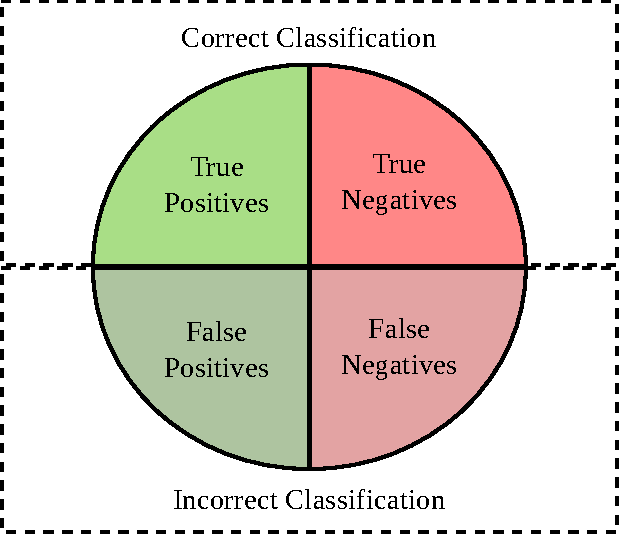
\includegraphics[scale=0.85]{src/background/figs/evaluation-classification.pdf}
  \caption{.}
  \label{fig:evaluation-classification}
\end{figure}
